\documentclass[t]{beamer}
\usepackage{textcomp}
\usepackage{caption}
\usepackage{listings}
\usepackage{amssymb}
\usepackage{minted}

\usetheme{default}
\usebackgroundtemplate{
\includegraphics[width=\paperwidth]{../cpeb_bkground_topleft.pdf}}

\setbeamertemplate{frametitle}{
  \centering\vspace{1mm}\insertframetitle\par\vspace{3mm}
}

\title{Lab chat on my PhD
  \subtitle{``Novel algorithms for population-scale analysis of complex
              plant genomes''}
\author{Kevin Murray}
\institute{Borevitz Lab, ANU}
\date{\today}
}

\begin{document}

{
\usebackgroundtemplate{
\includegraphics[width=\paperwidth]{../cpeb_bkground_centered.pdf}}
\begin{frame}
  \titlepage
  \vfill
\end{frame}
}

\begin{frame}{What?}
  \begin{itemize}
    \item Novel algorithms to analyse large-scale genomics data
  \pause
    \item Our wish-list:
    \begin{itemize}
      \item Reference \& alignment free
      \item Tolerates any sequencing platform
      \item Works with Borevitz-style ``wide and shallow'' expts: e.g. 1000
        samples at 1x
    \end{itemize}
  \end{itemize}
\end{frame}

\begin{frame}{How?}
  \begin{itemize}
    \item $k$-mer analysis: analyse $k$-length words of sequence
    \begin{itemize}
      \item Fast
      \item Constant-memory (with \texttt{khmer})
      \item Scaleable and parallelisable
    \end{itemize}
  \pause
    \item Multi-layered ``zooming'' analysis
      \begin{itemize}
        \item First pass basic clustering
        \item Error correction
        \item Population graph ``alignment''
        \item Variant calling
      \end{itemize}
  \pause
    \item In-silico experiment-driven development
  \end{itemize}
\end{frame}

\begin{frame}{What have I been up to}
  \begin{itemize}
    \item $k$-mer based clustering
  \pause
    \item In collaboration w/ Sylvain Foret, Cheng-Soon Ong, Christfried
      Webers (NICTA)
  \pause
    \item Extending work in alignment-free sequence comparison (SF) and
      text/document clustering (C-SO, CW @ NICTA).
  \pause
    \item Have functioning software package: \texttt{kWIP}
  \pause
    \item Using Titus Brown's \texttt{khmer} (contributed a lot of code myself)
  \end{itemize}
\end{frame}

\begin{frame}{\texttt{kWIP}}
  \begin{itemize}
    \item The k-mer Weighted Inner Product
    \pause
    \item Algorithm:
      \begin{itemize}
        \item For each sample: count all k-mers (k=20) into a hash
        \pause
        \item For each analysis set, a.k.a ``population'':
          \begin{itemize}
            \item Calculate the informational entropy of hash bins (vector $P$)
            \item For each pair of hashes $A$ and $B$, calculate $A \cdot B
                  \cdot P$
          \end{itemize}
      \end{itemize}
    \pause
  \end{itemize}
\end{frame}

\begin{frame}{Shannon Entropy}
  \begin{center}
    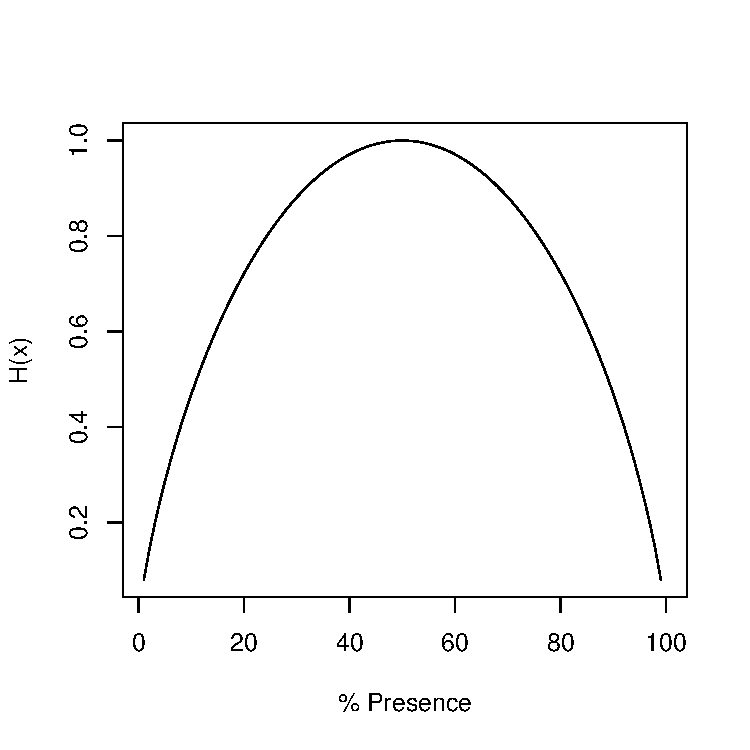
\includegraphics[width=0.7\textwidth]{img/shanent.pdf}
  \end{center}
\end{frame}

\begin{frame}{\texttt{kWIP}}
  \begin{itemize}
    \item The software:
      \begin{itemize}
        \item C++, 2000 SLOC
        \item Depends on \texttt{khmer}
        \item Parallelised, $\approx$ 12 hrs for 96 rice samples.
      \end{itemize}
    \pause
    \item The paper:
      \begin{itemize}
        \item Coming soon, planning to have it done by August
        \item Involves many in-silico experiments
      \end{itemize}
  \end{itemize}
\end{frame}


\begin{frame}{Rice Experiment}
  \begin{itemize}
    \item 3000 rice lines, 25k sequence runs, 20TB data
    \item Analysing in sets of 96, from two major groups
    \item Looks very accurate, detect Basmatia as Jap, strange samples.
  \end{itemize}
\end{frame}

\begin{frame}{Drosophila}
  \begin{itemize}
    \item Several read technologies
    \item Several species, population, reps
    \item Detect failed samples, repoduced known tree
  \end{itemize}
\end{frame}

\begin{frame}{Simulation??}
  \begin{itemize}
    \item Need to think about simulation
    \item Time consuming to do well, but can make lots of data
    \item Can we do it somewhat dodgy?
  \end{itemize}
\end{frame}

\end{document}
